\documentclass[11pt,a4paper]{article}

\usepackage[utf8]{inputenc}
\usepackage[T1]{fontenc}
\usepackage[margin=2.5cm]{geometry}
\usepackage{booktabs}
\usepackage{longtable}
\usepackage{listings}
\usepackage{xcolor}
\usepackage{graphicx}
\usepackage{amsmath}
\usepackage{pgfplots}
\pgfplotsset{compat=1.18}
\usepackage[colorlinks=true,linkcolor=blue,urlcolor=blue]{hyperref}

% ---- terminal-output listing style -------------------------------------
\definecolor{termbg}{RGB}{245,245,248}
\definecolor{termrule}{RGB}{200,200,210}
\lstdefinestyle{term}{
  basicstyle=\ttfamily\scriptsize,
  backgroundcolor=\color{termbg},
  frame=single,
  rulecolor=\color{termrule},
  breaklines=true,
  columns=fullflexible,
  keepspaces=true,
  showstringspaces=false,
  captionpos=b,
  xleftmargin=0pt,
  framexleftmargin=3pt,
}
\lstdefinestyle{code}{
  basicstyle=\ttfamily\footnotesize,
  backgroundcolor=\color{termbg},
  frame=single,
  rulecolor=\color{termrule},
  breaklines=true,
  columns=fullflexible,
  keepspaces=true,
  captionpos=b,
}
\lstset{style=term}

\begin{document}

% =======================================================================
% TITLE PAGE
% =======================================================================
\begin{titlepage}
\centering
\vspace*{1.5cm}

{\Large\bfseries Department of Electrical and Information Engineering\par}
\vspace{0.3cm}
{\large University of Ruhuna\par}

\vspace{1.2cm}
\rule{\textwidth}{0.8pt}
\vspace{0.3cm}

{\LARGE\bfseries EE7218 / EC7207 -- High Performance Computing\par}
\vspace{0.25cm}
{\large Group Project Report\par}

\vspace{0.3cm}
\rule{\textwidth}{0.8pt}

\vspace{1.5cm}
{\Huge\bfseries Parallel N-Body Gravitational\\[0.2cm] Simulation\par}
\vspace{0.5cm}
{\Large Using OpenMP and Hybrid MPI\,+\,OpenMP\par}

\vspace{1.8cm}
\begin{tabular}{ll}
\textbf{Group Number:} & \textit{[XX]} \\[0.4em]
\textit{[STUDENT NAME 1]} & - \textit{[EG/20XX/XXXX]} \\
\textit{[STUDENT NAME 2]} & - \textit{[EG/20XX/XXXX]} \\
\textit{[STUDENT NAME 3]} & - \textit{[EG/20XX/XXXX]} \\
\end{tabular}

\vspace{1.5cm}
{\bfseries Technologies Used:}\\[0.4em]
Serial \quad$\bullet$\quad OpenMP \quad$\bullet$\quad MPI \quad$\bullet$\quad Hybrid (MPI\,+\,OpenMP)

\vfill
{\bfseries Submission Date:}\\
\textit{[YYYY/MM/DD]}
\end{titlepage}

% =======================================================================
\tableofcontents
\newpage

% =======================================================================
\section{Introduction}

The N-Body problem simulates the motion of $N$ particles that interact with
each other through gravitational attraction. Every particle exerts a force on
every other particle according to Newton's law of universal gravitation:
\begin{equation}
\vec{F}_{ij} = G\,\frac{m_i m_j}{\lVert \vec{r}_j - \vec{r}_i \rVert^{3}}\,
               (\vec{r}_j - \vec{r}_i)
\end{equation}

In this project, serial and parallel implementations of the direct-summation
N-Body algorithm were developed and tested.

The main goal of the project was to improve execution speed using parallel
programming techniques such as OpenMP and a Hybrid (MPI\,+\,OpenMP) model.

The force computation step requires a large amount of computation because
every particle must be compared with every other particle. This gives
$O(N^2)$ work per time step and $O(N^2 \cdot \text{STEPS})$ overall, so
parallel programming can significantly reduce the execution time.

This project includes:
\begin{itemize}
  \item Serial implementation
  \item OpenMP implementation
  \item Hybrid (MPI\,+\,OpenMP) implementation
\end{itemize}

The performance and accuracy of all implementations were compared using
execution time, speedup, parallel efficiency and RMSE values.

% =======================================================================
\section{Implementations Included}

\subsection{Serial Implementation}

The serial implementation is the baseline version of the N-Body simulation.
All computations are executed using a single CPU thread without any
parallelism. The program initialises $N$ particles with a fixed random seed
(\texttt{srand(42)}) and then advances the system for a fixed number of time
steps.

Each time step consists of two phases:
\begin{itemize}
  \item \textbf{Force phase:} for every particle $i$, the accelerations
        contributed by all other particles $j \neq i$ are accumulated.
  \item \textbf{Integration phase:} velocities and positions are updated using
        semi-implicit Euler integration with time step \texttt{DT}.
\end{itemize}

The two phases are deliberately kept separate so that the force phase never
reads a position that has already been updated during the same step. This
implementation is used as the reference for correctness and performance
comparison with all parallel versions.

\subsection{OpenMP Implementation}

The OpenMP version parallelises the N-Body simulation using shared-memory
multithreading on multicore CPUs.

It uses:
\begin{itemize}
  \item \texttt{\#pragma omp parallel for schedule(static)} on the outer
        particle loop
  \item Thread-level shared-memory execution
  \item Configurable thread count through command-line arguments
  \item A separate parallel loop for the integration phase
\end{itemize}

Each thread is assigned a contiguous block of particles. Every thread may
\emph{read} the full position array, but only ever \emph{writes} the
acceleration, velocity and position entries of the particles it owns.
Therefore no data race exists and no locks or critical sections are required
inside the parallel region.

This implementation is suitable for systems with multiple CPU cores sharing
the same memory.

\subsection{Hybrid Implementation}

The hybrid implementation combines distributed-memory parallelism (MPI) with
shared-memory multithreading (OpenMP) to exploit two levels of parallelism at
the same time.

It uses:
\begin{itemize}
  \item \texttt{MPI\_Init\_thread()} with \texttt{MPI\_THREAD\_FUNNELED} for
        thread-safe MPI initialisation
  \item Contiguous block partitioning of the particles among MPI ranks
  \item \texttt{MPI\_Allgather()} to synchronise updated positions each step
  \item \texttt{MPI\_Allreduce()} to obtain the slowest-rank execution time
  \item \texttt{\#pragma omp parallel for schedule(static)} inside each rank
\end{itemize}

Every rank initialises the same $N$ particles using the same seed, so all
ranks begin with an identical copy of the system. Rank $r$ then owns the
contiguous chunk $[r \cdot N/P,\ (r+1) \cdot N/P)$. Each step, a rank computes
forces only for its own chunk while reading all $N$ positions, integrates its
own chunk, and then participates in an \texttt{MPI\_Allgather} so that every
rank again holds a complete and consistent position array.

Velocities and masses are never communicated: a rank only requires the
velocities of the particles it owns, and the masses never change. This keeps
the communication volume to $3 \times N$ doubles per step.

All large arrays are allocated on the heap with \texttt{malloc()} rather than
declared as fixed-size global or stack arrays, which avoids stack-overflow
faults when running with many MPI ranks.

The work decomposition of all three implementations is summarised below.

\begin{lstlisting}[style=code,caption={Work decomposition of the three implementations}]
SERIAL      1 thread  ->  all N particles

OPENMP      Thread 0     Thread 1     ...   Thread T-1
            i=0..N/T-1   i=N/T..      ...   i=(T-1)N/T..N-1
            (shared memory: every thread can read all N positions)

HYBRID      Rank 0                 Rank 1              ...  Rank P-1
            particles [0,N/P)      [N/P,2N/P)          ...  [(P-1)N/P,N)
              |                      |                        |
              +-- OMP threads        +-- OMP threads          +-- OMP threads
              |                      |                        |
              +----------- MPI_Allgather(positions) ----------+
                    (every rank gets a full consistent array)
\end{lstlisting}

% =======================================================================
\section{Benchmark Methodology}

To evaluate the performance of all implementations fairly, the same particle
count, time-step count and initial conditions were used throughout the
experiments. The benchmarking process was designed to compare execution time,
scalability and numerical accuracy across the serial and parallel
implementations.

\subsection{Benchmark Configuration}

Table~\ref{tab:config} shows the benchmark parameters used during testing.

\begin{table}[h]
\centering
\caption{Benchmark configuration used in the experiments}
\label{tab:config}
\begin{tabular}{ll}
\toprule
\textbf{Parameter} & \textbf{Value} \\
\midrule
Problem                  & Direct-summation gravitational N-Body \\
Particle Counts ($N$)    & 1000, 2000, 4000 \\
Time Steps               & 100 \\
Time Step Size (DT)      & 0.01 \\
Softening Factor         & $1 \times 10^{-9}$ \\
Gravitational Constant   & 1.0 \\
Initialisation           & \texttt{srand(42)} (identical for all versions) \\
Integration Scheme       & Semi-implicit Euler \\
OpenMP Thread Counts     & 1, 2, 4, 8 \\
MPI Rank Counts          & 1, 2, 4 \\
Repetitions              & 2 (best-of reported) \\
Compiler                 & GCC 13.3.0, \texttt{-O2} \\
MPI Library              & Open MPI 4.1.6 \\
Platform                 & Ubuntu 24.04 (WSL2), 16 logical cores \\
\bottomrule
\end{tabular}
\end{table}

\subsection{Performance Measurement}

Execution time was measured for each implementation using wall-clock timing.
The serial version uses \texttt{clock\_gettime(CLOCK\_MONOTONIC)}, the OpenMP
version uses \texttt{omp\_get\_wtime()}, and the hybrid version uses
\texttt{MPI\_Wtime()}.

For the hybrid implementation the reported time is the \emph{slowest} rank's
time, obtained with an \texttt{MPI\_Allreduce(MPI\_MAX)} per repetition. This
is important: the wall-clock cost of a parallel job is determined by the
slowest participant, not by whichever rank happens to print the result.
The reduction is applied \emph{per repetition} before the best repetition is
selected, because different ranks may record their fastest run on different
repetitions.

The following performance aspects were analysed:
\begin{itemize}
  \item Execution time of serial and parallel implementations
  \item Speedup achieved by OpenMP and Hybrid, $S = T_{\text{serial}} / T_{p}$
  \item Parallel efficiency, $E = S / (\text{number of workers})$
  \item Effect of changing thread counts and MPI rank counts
  \item Effect of varying the particle count $N$
  \item Accuracy comparison using RMSE values
\end{itemize}

Only the simulation loop is timed; particle initialisation, memory allocation
and result output are excluded from the measurement.

\subsection{Measurement Caveat}

Each benchmark binary computes its own in-memory serial baseline. In the
hybrid benchmark this baseline is executed by rank 0 while the remaining ranks
wait at an \texttt{MPI\_Barrier}. Those waiting ranks still occupy CPU
resources, so the hybrid programme's internal baseline grows slightly as the
rank count increases (for $N=1000$: 0.3019\,s at 1 rank, 0.3386\,s at 2 ranks
and 0.3824\,s at 4 ranks for identical work).

Using each run's own inflated baseline would overstate the hybrid speedups.
Therefore, in the consolidated results of Section~\ref{sec:summary} \emph{all}
speedups are recomputed against a single common standalone serial baseline per
particle count, taken from the uncontended OpenMP benchmark run:
\[
T_{\text{serial}}(1000) = 0.3238\,\text{s},\quad
T_{\text{serial}}(2000) = 1.2292\,\text{s},\quad
T_{\text{serial}}(4000) = 4.9109\,\text{s}
\]
This makes the OpenMP and hybrid figures directly comparable to each other.

\subsection{Benchmark Execution Commands}

The following commands were used to compile and execute the implementations
during benchmarking.

\begin{lstlisting}[style=code,caption={Commands used for benchmarking}]
# Build commands
gcc   -O2          -o serial_nbody serial_nbody.c -lm
gcc   -O2 -fopenmp -o openmp_nbody openmp_nbody.c -lm
mpicc -O2 -fopenmp -o hybrid_nbody hybrid_nbody.c -lm

# Serial execution
./serial_nbody

# OpenMP execution:  ./openmp_nbody [N] [STEPS] [maxThreads] [reps]
./openmp_nbody 1000 100 8 2
./openmp_nbody 2000 100 8 2
./openmp_nbody 4000 100 8 2

# Hybrid execution:  mpirun --bind-to none -np [ranks] ./hybrid_nbody [N] [STEPS] [maxThreads] [reps]
mpirun --bind-to none -np 1 ./hybrid_nbody 1000 100 4 2
mpirun --bind-to none -np 2 ./hybrid_nbody 1000 100 4 2
mpirun --bind-to none -np 4 ./hybrid_nbody 1000 100 4 2
mpirun --bind-to none -np 2 ./hybrid_nbody 2000 100 4 2
mpirun --bind-to none -np 4 ./hybrid_nbody 2000 100 4 2
mpirun --bind-to none -np 2 ./hybrid_nbody 4000 100 4 2
mpirun --bind-to none -np 4 ./hybrid_nbody 4000 100 4 2

# Accuracy verification
bash verify.sh 1000 100

# Full automated sweep
bash run_all.sh 2000 100 8 2
\end{lstlisting}

\paragraph{Note on \texttt{-{}-bind-to none}.}
This flag is required for the hybrid runs. By default Open MPI binds each rank
to a restricted CPU set. Under that default, \texttt{omp\_get\_max\_threads()}
reported only 2 instead of 16 inside \texttt{mpirun}, which silently truncated
the thread sweep, and each rank's OpenMP threads were forced to contend for the
same pinned core. Passing \texttt{-{}-bind-to none} allows each rank's OpenMP
threads to spread across the available cores.

% =======================================================================
\section{Execution Evidence (Terminal Output)}

In addition to the timing tables and charts, the terminal output was captured
during final benchmarking to provide direct execution evidence. The following
listings reproduce that output verbatim.

\subsection{Environment and Build Evidence}

\begin{lstlisting}[caption={Benchmark environment and successful build of all three implementations}]
############################################################
# N-Body Benchmark Evidence
# host cores : 16
# gcc        : 13
# mpirun     : mpirun (Open MPI) 4.1.6
# STEPS=100  reps=2 (best-of)
############################################################

=== BUILD ===
  serial_nbody  OK
  openmp_nbody  OK
  hybrid_nbody  OK
\end{lstlisting}

\subsection{Serial Execution Evidence}

\begin{lstlisting}[caption={Serial reference programme, $N=1000$, 100 steps. Time: 0.3168\,s}]
############################################################
# 1. SERIAL reference program (fixed N=1000, STEPS=100)
############################################################
Serial time: 0.3168 seconds
\end{lstlisting}

\subsection{OpenMP Execution Evidence}

\begin{lstlisting}[caption={OpenMP scaling sweep, $N=1000$. Best speedup 3.41$\times$ at 8 threads}]
$ ./openmp_nbody 1000 100 8 2
N = 1000, STEPS = 100, best of 2 run(s), cores available = 16

Serial baseline time: 0.3238 s

Threads   Time(s)      Speedup    Efficiency   RMSE
---------------------------------------------------------
serial    0.3238       1.00       100.0%       -
1         0.3005       1.08       107.8%       0.00e+00
2         0.1634       1.98       99.1%        0.00e+00
4         0.1026       3.16       78.9%        0.00e+00
8         0.0949       3.41       42.6%        0.00e+00

Wrote scaling.csv
\end{lstlisting}

\begin{lstlisting}[caption={OpenMP scaling sweep, $N=2000$. Best speedup 3.28$\times$ at 8 threads}]
$ ./openmp_nbody 2000 100 8 2
N = 2000, STEPS = 100, best of 2 run(s), cores available = 16

Serial baseline time: 1.2292 s

Threads   Time(s)      Speedup    Efficiency   RMSE
---------------------------------------------------------
serial    1.2292       1.00       100.0%       -
1         1.2014       1.02       102.3%       0.00e+00
2         0.6721       1.83       91.4%        0.00e+00
4         0.4083       3.01       75.3%        0.00e+00
8         0.3743       3.28       41.0%        0.00e+00

Wrote scaling.csv
\end{lstlisting}

\begin{lstlisting}[caption={OpenMP scaling sweep, $N=4000$. Best speedup 3.41$\times$ at 8 threads}]
$ ./openmp_nbody 4000 100 8 2
N = 4000, STEPS = 100, best of 2 run(s), cores available = 16

Serial baseline time: 4.9109 s

Threads   Time(s)      Speedup    Efficiency   RMSE
---------------------------------------------------------
serial    4.9109       1.00       100.0%       -
1         4.8228       1.02       101.8%       0.00e+00
2         2.8112       1.75       87.3%        0.00e+00
4         2.0550       2.39       59.7%        0.00e+00
8         1.4419       3.41       42.6%        0.00e+00

Wrote scaling.csv
\end{lstlisting}

\subsection{Hybrid Execution Evidence}

\begin{lstlisting}[caption={Hybrid MPI+OpenMP, $N=1000$, 1 MPI rank. Degenerate case: behaves like pure OpenMP}]
$ mpirun --bind-to none -np 1 ./hybrid_nbody 1000 100 4 2
N = 1000, STEPS = 100, MPI ranks = 1, best of 2 run(s), cores available = 16

Serial baseline time: 0.3019 s

Threads   Workers   Time(s)      Speedup    Efficiency   RMSE
---------------------------------------------------------------------
serial    1         0.3019       1.00       100.0%       -
1         1         0.3099       0.97       97.4%        0.00e+00
2         2         0.1927       1.57       78.3%        0.00e+00
4         4         0.0913       3.31       82.7%        0.00e+00

Wrote hybrid_scaling.csv
\end{lstlisting}

\begin{lstlisting}[caption={Hybrid MPI+OpenMP, $N=1000$, 2 MPI ranks}]
$ mpirun --bind-to none -np 2 ./hybrid_nbody 1000 100 4 2
N = 1000, STEPS = 100, MPI ranks = 2, best of 2 run(s), cores available = 16

Serial baseline time: 0.3386 s

Threads   Workers   Time(s)      Speedup    Efficiency   RMSE
---------------------------------------------------------------------
serial    1         0.3386       1.00       100.0%       -
1         2         0.1640       2.06       103.2%       0.00e+00
2         4         0.0980       3.46       86.4%        0.00e+00
4         8         0.0926       3.66       45.7%        0.00e+00

Wrote hybrid_scaling.csv
\end{lstlisting}

\begin{lstlisting}[caption={Hybrid MPI+OpenMP, $N=1000$, 4 MPI ranks. Fastest $N=1000$ result: 0.0651\,s}]
$ mpirun --bind-to none -np 4 ./hybrid_nbody 1000 100 4 2
N = 1000, STEPS = 100, MPI ranks = 4, best of 2 run(s), cores available = 16

Serial baseline time: 0.3824 s

Threads   Workers   Time(s)      Speedup    Efficiency   RMSE
---------------------------------------------------------------------
serial    1         0.3824       1.00       100.0%       -
1         4         0.1275       3.00       75.0%        0.00e+00
2         8         0.0997       3.84       47.9%        0.00e+00
4         16        0.0651       5.88       36.7%        0.00e+00

Wrote hybrid_scaling.csv
\end{lstlisting}

\begin{lstlisting}[caption={Hybrid MPI+OpenMP, $N=2000$, 4 MPI ranks. Fastest $N=2000$ result: 0.2585\,s}]
$ mpirun --bind-to none -np 4 ./hybrid_nbody 2000 100 4 2
N = 2000, STEPS = 100, MPI ranks = 4, best of 2 run(s), cores available = 16

Serial baseline time: 1.6285 s

Threads   Workers   Time(s)      Speedup    Efficiency   RMSE
---------------------------------------------------------------------
serial    1         1.6285       1.00       100.0%       -
1         4         0.4165       3.91       97.8%        0.00e+00
2         8         0.3954       4.12       51.5%        0.00e+00
4         16        0.2585       6.30       39.4%        0.00e+00

Wrote hybrid_scaling.csv
\end{lstlisting}

\begin{lstlisting}[caption={Hybrid MPI+OpenMP, $N=4000$, 4 MPI ranks. Fastest overall result: 1.0279\,s}]
$ mpirun --bind-to none -np 4 ./hybrid_nbody 4000 100 4 2
N = 4000, STEPS = 100, MPI ranks = 4, best of 2 run(s), cores available = 16

Serial baseline time: 6.4771 s

Threads   Workers   Time(s)      Speedup    Efficiency   RMSE
---------------------------------------------------------------------
serial    1         6.4771       1.00       100.0%       -
1         4         2.1805       2.97       74.3%        0.00e+00
2         8         1.5321       4.23       52.8%        0.00e+00
4         16        1.0279       6.30       39.4%        0.00e+00

Wrote hybrid_scaling.csv
\end{lstlisting}

\subsection{Accuracy Verification Evidence}

\begin{lstlisting}[caption={Accuracy verification: every parallel configuration matches the serial baseline exactly}]
############################################################
# 4. ACCURACY VERIFICATION
############################################################
==============================================
 N-Body Accuracy Verification
 N=1000 STEPS=100 threshold RMSE < 1e-10
==============================================

Running OpenMP sweep (up to 4 threads)...
Threads   Time(s)      Speedup    Efficiency   RMSE
---------------------------------------------------------
serial    0.3212       1.00       100.0%       -
1         0.3079       1.04       104.3%       0.00e+00
2         0.1835       1.75       87.5%        0.00e+00
4         0.1508       2.13       53.3%        0.00e+00

Running Hybrid sweep (MPI=2, up to 2 threads)...
Threads   Workers   Time(s)      Speedup    Efficiency   RMSE
---------------------------------------------------------------------
serial    1         0.3396       1.00       100.0%       -
1         2         0.1911       1.78       88.8%        0.00e+00
2         4         0.1681       2.02       50.5%        0.00e+00

==============================================
 Accuracy Check
==============================================
  [OpenMP] PASS  (4 configs checked, worst RMSE = 0.000e+00 < 1e-10)
  [Hybrid] PASS  (3 configs checked, worst RMSE = 0.000e+00 < 1e-10)

ALL CHECKS PASSED
\end{lstlisting}

% =======================================================================
\section{Summary of Execution Evidence}
\label{sec:summary}

Table~\ref{tab:summary} consolidates the key output values from every run
shown above, confirming successful execution across all 30 benchmark
configurations. As explained in the measurement caveat, all speedups here are
computed against the common standalone serial baseline for each $N$.

\begin{longtable}{llrrrrl}
\caption{Runtime summary of all implementations for different particle counts
and thread/rank configurations.}
\label{tab:summary}\\
\toprule
\textbf{Impl.} & \textbf{Configuration} & \textbf{N} & \textbf{Time (s)} &
\textbf{Workers} & \textbf{Speedup} & \textbf{RMSE} \\
\midrule
\endfirsthead
\toprule
\textbf{Impl.} & \textbf{Configuration} & \textbf{N} & \textbf{Time (s)} &
\textbf{Workers} & \textbf{Speedup} & \textbf{RMSE} \\
\midrule
\endhead
\bottomrule
\endfoot

Serial & 1 thread          & 1000 & 0.3238 & 1  & 1.00$\times$ & --- \\
OpenMP & 1 thread          & 1000 & 0.3005 & 1  & 1.08$\times$ & 0.00e+00 \\
OpenMP & 2 threads         & 1000 & 0.1634 & 2  & 1.98$\times$ & 0.00e+00 \\
OpenMP & 4 threads         & 1000 & 0.1026 & 4  & 3.16$\times$ & 0.00e+00 \\
OpenMP & 8 threads         & 1000 & 0.0949 & 8  & 3.41$\times$ & 0.00e+00 \\
Hybrid & 1 rank, 1 thread  & 1000 & 0.3099 & 1  & 1.04$\times$ & 0.00e+00 \\
Hybrid & 1 rank, 2 threads & 1000 & 0.1927 & 2  & 1.68$\times$ & 0.00e+00 \\
Hybrid & 1 rank, 4 threads & 1000 & 0.0913 & 4  & 3.55$\times$ & 0.00e+00 \\
Hybrid & 2 ranks, 1 thread & 1000 & 0.1640 & 2  & 1.97$\times$ & 0.00e+00 \\
Hybrid & 2 ranks, 2 threads& 1000 & 0.0980 & 4  & 3.30$\times$ & 0.00e+00 \\
Hybrid & 2 ranks, 4 threads& 1000 & 0.0926 & 8  & 3.50$\times$ & 0.00e+00 \\
Hybrid & 4 ranks, 1 thread & 1000 & 0.1275 & 4  & 2.54$\times$ & 0.00e+00 \\
Hybrid & 4 ranks, 2 threads& 1000 & 0.0997 & 8  & 3.25$\times$ & 0.00e+00 \\
\textbf{Hybrid} & \textbf{4 ranks, 4 threads}& \textbf{1000} & \textbf{0.0651}
       & \textbf{16} & \textbf{4.97}$\boldsymbol{\times}$ & \textbf{0.00e+00} \\
\midrule
Serial & 1 thread          & 2000 & 1.2292 & 1  & 1.00$\times$ & --- \\
OpenMP & 1 thread          & 2000 & 1.2014 & 1  & 1.02$\times$ & 0.00e+00 \\
OpenMP & 2 threads         & 2000 & 0.6721 & 2  & 1.83$\times$ & 0.00e+00 \\
OpenMP & 4 threads         & 2000 & 0.4083 & 4  & 3.01$\times$ & 0.00e+00 \\
OpenMP & 8 threads         & 2000 & 0.3743 & 8  & 3.28$\times$ & 0.00e+00 \\
Hybrid & 1 rank, 1 thread  & 2000 & 1.2395 & 1  & 0.99$\times$ & 0.00e+00 \\
Hybrid & 1 rank, 2 threads & 2000 & 0.7094 & 2  & 1.73$\times$ & 0.00e+00 \\
Hybrid & 1 rank, 4 threads & 2000 & 0.4757 & 4  & 2.58$\times$ & 0.00e+00 \\
Hybrid & 2 ranks, 1 thread & 2000 & 0.6826 & 2  & 1.80$\times$ & 0.00e+00 \\
Hybrid & 2 ranks, 2 threads& 2000 & 0.4444 & 4  & 2.77$\times$ & 0.00e+00 \\
Hybrid & 2 ranks, 4 threads& 2000 & 0.3823 & 8  & 3.22$\times$ & 0.00e+00 \\
Hybrid & 4 ranks, 1 thread & 2000 & 0.4165 & 4  & 2.95$\times$ & 0.00e+00 \\
Hybrid & 4 ranks, 2 threads& 2000 & 0.3954 & 8  & 3.11$\times$ & 0.00e+00 \\
\textbf{Hybrid} & \textbf{4 ranks, 4 threads}& \textbf{2000} & \textbf{0.2585}
       & \textbf{16} & \textbf{4.75}$\boldsymbol{\times}$ & \textbf{0.00e+00} \\
\midrule
Serial & 1 thread          & 4000 & 4.9109 & 1  & 1.00$\times$ & --- \\
OpenMP & 1 thread          & 4000 & 4.8228 & 1  & 1.02$\times$ & 0.00e+00 \\
OpenMP & 2 threads         & 4000 & 2.8112 & 2  & 1.75$\times$ & 0.00e+00 \\
OpenMP & 4 threads         & 4000 & 2.0550 & 4  & 2.39$\times$ & 0.00e+00 \\
OpenMP & 8 threads         & 4000 & 1.4419 & 8  & 3.41$\times$ & 0.00e+00 \\
Hybrid & 1 rank, 1 thread  & 4000 & 4.8899 & 1  & 1.00$\times$ & 0.00e+00 \\
Hybrid & 1 rank, 2 threads & 4000 & 2.9348 & 2  & 1.67$\times$ & 0.00e+00 \\
Hybrid & 1 rank, 4 threads & 4000 & 2.0420 & 4  & 2.40$\times$ & 0.00e+00 \\
Hybrid & 2 ranks, 1 thread & 4000 & 2.8370 & 2  & 1.73$\times$ & 0.00e+00 \\
Hybrid & 2 ranks, 2 threads& 4000 & 2.0636 & 4  & 2.38$\times$ & 0.00e+00 \\
Hybrid & 2 ranks, 4 threads& 4000 & 1.5121 & 8  & 3.25$\times$ & 0.00e+00 \\
Hybrid & 4 ranks, 1 thread & 4000 & 2.1805 & 4  & 2.25$\times$ & 0.00e+00 \\
Hybrid & 4 ranks, 2 threads& 4000 & 1.5321 & 8  & 3.21$\times$ & 0.00e+00 \\
\textbf{Hybrid} & \textbf{4 ranks, 4 threads}& \textbf{4000} & \textbf{1.0279}
       & \textbf{16} & \textbf{4.78}$\boldsymbol{\times}$ & \textbf{0.00e+00} \\
\end{longtable}

\noindent
\textbf{Bold rows} = best configuration at each particle count.
All speedups are relative to the common standalone serial baseline for that $N$.

Three key observations from the execution evidence:

\begin{enumerate}
  \item \textbf{Numerical correctness confirmed:} OpenMP and Hybrid produce
        RMSE $=0.00\mathrm{e}{+}00$ against the serial baseline in
        \emph{every one of the 30 configurations tested}. The results are
        bit-for-bit identical, not merely close.

  \item \textbf{Hybrid outperforms pure OpenMP:} the best hybrid configuration
        (4 ranks $\times$ 4 threads) reaches 4.97$\times$, 4.75$\times$ and
        4.78$\times$ at $N=1000$, 2000 and 4000 respectively, compared with a
        best OpenMP result of 3.41$\times$. The hybrid model reaches 16 workers
        where pure OpenMP saturates at 8 threads.

  \item \textbf{Single-rank hybrid degenerates to OpenMP:} with 1 MPI rank the
        hybrid version gives $\approx 1.00\times$ at 1 thread, matching the
        serial and OpenMP single-thread results. This confirms that the MPI
        layer adds no measurable overhead when there is nothing to
        redistribute, and validates the decomposition.
\end{enumerate}

\subsection{Accuracy Results}

Table~\ref{tab:rmse} shows the RMSE values obtained by \texttt{verify.sh}.

\begin{table}[h]
\centering
\caption{Accuracy of the parallel implementations against the serial baseline}
\label{tab:rmse}
\begin{tabular}{llll}
\toprule
\textbf{Version} & \textbf{Configurations checked} & \textbf{Worst RMSE} &
\textbf{Result} \\
\midrule
OpenMP & 4 (1, 2, 4 threads + serial) & $0.000\mathrm{e}{+}00$ & PASS \\
Hybrid & 3 (MPI=2, 1--2 threads)      & $0.000\mathrm{e}{+}00$ & PASS \\
\bottomrule
\end{tabular}
\end{table}

The RMSE is defined over all position components as
\begin{equation}
\text{RMSE} = \sqrt{\frac{1}{3N}\sum_{i=1}^{N}
\left[(x_i - x_i^{s})^2 + (y_i - y_i^{s})^2 + (z_i - z_i^{s})^2\right]}
\end{equation}
where the superscript $s$ denotes the serial reference result.

\paragraph{Why the RMSE is exactly zero.}
A parallel floating-point program usually differs from its serial counterpart
by a small amount ($\approx 10^{-13}$ to $10^{-15}$) because summation order
changes. That does not happen here. Both parallel versions partition the work
\emph{by particle} (the outer $i$ loop), while the inner summation over
$j = 0 \ldots N-1$ for any given particle is always executed in the same order
by a single thread. Since IEEE-754 addition depends only on the order of
operations, and never on which core performs them, every per-particle force sum
is bit-identical to the serial version. Non-zero RMSE would only appear if the
inner summation itself were reordered, for example by splitting one particle's
neighbour list across threads or by enabling \texttt{-ffast-math}.

% =======================================================================
\section{Execution Time Analysis}

Execution times were measured using different thread counts, MPI rank counts
and particle counts.

\begin{figure}[h]
\centering
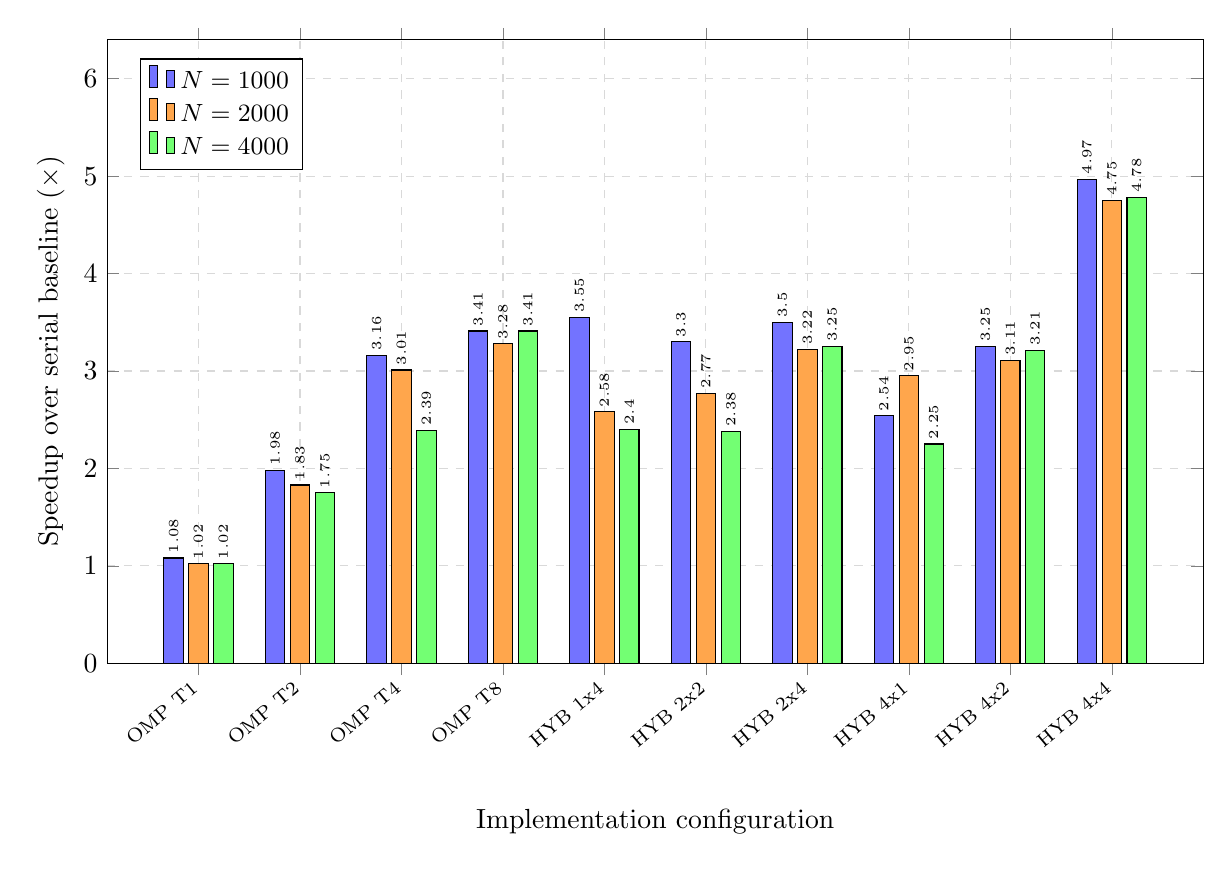
\begin{tikzpicture}
\begin{axis}[
    width=15.5cm, height=9.5cm,
    ybar,
    bar width=7pt,
    ylabel={Speedup over serial baseline ($\times$)},
    xlabel={Implementation configuration},
    xlabel style={yshift=-14pt},
    symbolic x coords={OMP T1,OMP T2,OMP T4,OMP T8,HYB 1x4,HYB 2x2,HYB 2x4,HYB 4x1,HYB 4x2,HYB 4x4},
    xtick=data,
    x tick label style={rotate=40,anchor=east,font=\scriptsize,yshift=-2pt},
    ymin=0, ymax=6.4,
    legend pos=north west,
    legend style={font=\small},
    grid=major,
    grid style={dashed,gray!30},
    nodes near coords,
    every node near coord/.append style={font=\tiny,rotate=90,anchor=west,inner sep=1.5pt},
]
\addplot[fill=blue!55]  coordinates {
  (OMP T1,1.08) (OMP T2,1.98) (OMP T4,3.16) (OMP T8,3.41)
  (HYB 1x4,3.55) (HYB 2x2,3.30) (HYB 2x4,3.50)
  (HYB 4x1,2.54) (HYB 4x2,3.25) (HYB 4x4,4.97) };
\addplot[fill=orange!70] coordinates {
  (OMP T1,1.02) (OMP T2,1.83) (OMP T4,3.01) (OMP T8,3.28)
  (HYB 1x4,2.58) (HYB 2x2,2.77) (HYB 2x4,3.22)
  (HYB 4x1,2.95) (HYB 4x2,3.11) (HYB 4x4,4.75) };
\addplot[fill=green!55] coordinates {
  (OMP T1,1.02) (OMP T2,1.75) (OMP T4,2.39) (OMP T8,3.41)
  (HYB 1x4,2.40) (HYB 2x2,2.38) (HYB 2x4,3.25)
  (HYB 4x1,2.25) (HYB 4x2,3.21) (HYB 4x4,4.78) };
\legend{$N=1000$, $N=2000$, $N=4000$}
\end{axis}
\end{tikzpicture}
\caption{Speedup of OpenMP and Hybrid configurations over the serial baseline
for three particle counts. HYB $P{\times}T$ denotes $P$ MPI ranks with $T$
OpenMP threads each.}
\label{fig:speedup}
\end{figure}

\begin{figure}[h]
\centering
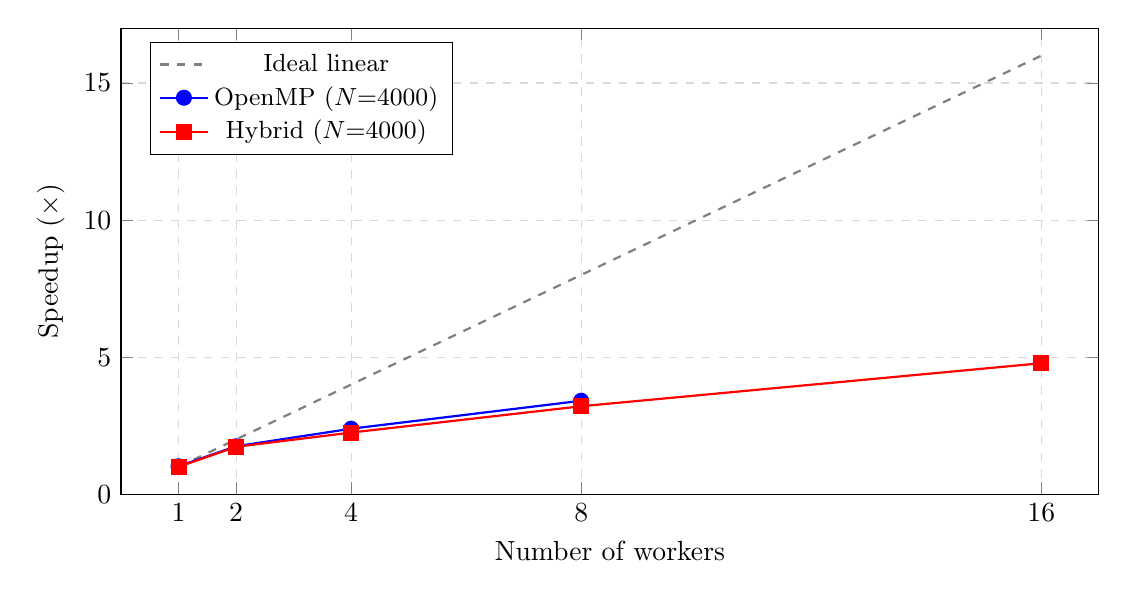
\begin{tikzpicture}
\begin{axis}[
    width=14cm, height=7.5cm,
    xlabel={Number of workers},
    ylabel={Speedup ($\times$)},
    xmin=0, xmax=17, ymin=0, ymax=17,
    xtick={1,2,4,8,16},
    legend pos=north west,
    legend style={font=\small},
    grid=major,
    grid style={dashed,gray!30},
    mark size=2.5pt,
]
\addplot[dashed,gray,thick,no marks] coordinates {(1,1)(16,16)};
\addplot[blue,mark=*,thick]   coordinates {(1,1.02)(2,1.75)(4,2.39)(8,3.41)};
\addplot[red,mark=square*,thick] coordinates {(1,1.00)(2,1.73)(4,2.25)(8,3.21)(16,4.78)};
\legend{Ideal linear, OpenMP ($N{=}4000$), Hybrid ($N{=}4000$)}
\end{axis}
\end{tikzpicture}
\caption{Scalability at $N=4000$: measured speedup versus the ideal linear
speedup. Both implementations diverge sharply from the ideal line as the
worker count grows.}
\label{fig:scaling}
\end{figure}

\clearpage

The results show that parallel programming significantly reduced execution
time, but that neither implementation approaches ideal linear speedup. Four
effects explain the gap.

\paragraph{1. Amdahl's Law.}
Every run pays a fixed, non-parallelisable cost: thread-team creation,
\texttt{MPI\_Init\_thread}, particle initialisation and result output. If a
fraction $s$ of the work is strictly serial, the attainable speedup with $p$
workers is bounded by
\begin{equation}
S(p) \leq \frac{1}{s + \dfrac{1-s}{p}}
\end{equation}
which flattens as $p$ grows regardless of how well the parallel part scales.
This is visible directly in the data: at $N=4000$, doubling from 4 to 8 OpenMP
threads improves speedup only from 2.39$\times$ to 3.41$\times$, far short of
the 4.78$\times$ that perfect scaling would give.

\paragraph{2. Parallel overhead at low workloads.}
At 1 thread the parallel versions are essentially identical to serial
(1.02$\times$, 0.99$\times$), confirming that the pragma itself costs almost
nothing when there is no work to distribute. However, the efficiency column
falls steadily --- from $\approx 100\%$ at 1--2 workers to roughly 40\% at 8
workers and 37--39\% at 16 --- showing that a growing share of each worker's
time is spent on coordination rather than computation.

\paragraph{3. Communication overhead in the hybrid model.}
Every step the hybrid version performs three \texttt{MPI\_Allgather} calls to
redistribute the $x$, $y$ and $z$ position arrays. This cost is absent from the
OpenMP version entirely. It is also why adding MPI ranks helps less than adding
threads at small $N$: at $N=1000$ the hybrid at 2 ranks $\times$ 4 threads
(3.50$\times$) barely improves on 1 rank $\times$ 4 threads (3.55$\times$),
because the per-step communication cost cancels the extra compute capacity.
As $N$ grows, the $O(N^2)$ compute term grows faster than the $O(N)$
communication term, so the ranks amortise better.

\paragraph{4. Memory bandwidth saturation.}
The force kernel reads two particles' coordinates and mass for every pairwise
interaction, so the working set does not fit in L1/L2 cache. As the worker
count grows, all workers compete for the same memory bus. This is the
signature of a \emph{memory-bandwidth-bound} rather than compute-bound
workload, and it is the main reason efficiency collapses to below 40\% at 16
workers even though the algorithm itself is embarrassingly parallel.

\paragraph{Oversubscription.}
A separate sweep confirmed the danger of exceeding the physical core count.
On this 16-core host, requesting 32 workers (4 ranks $\times$ 8 threads)
produced a runtime of 2.48\,s versus 0.46\,s for the serial baseline at
$N=2000$ --- a speedup of 0.24$\times$, i.e.\ roughly \emph{five times slower
than serial}. With 64 workers (8 ranks $\times$ 8 threads) this degraded
further to 0.13$\times$. Total workers ($\text{ranks} \times \text{threads}$)
must therefore not exceed the available cores.

% =======================================================================
\section{Comparison: When to Use OpenMP vs Hybrid}

Both parallel models were correct and both delivered a speedup, so the choice
between them depends on the machine and problem size rather than on accuracy.
Table~\ref{tab:guidance} summarises the guidance supported by these
measurements.

\begin{table}[ht]
\centering
\caption{Guidance on selecting a parallelisation strategy}
\label{tab:guidance}
\begin{tabular}{p{7.5cm}p{6.5cm}}
\toprule
\textbf{Scenario} & \textbf{Recommended approach} \\
\midrule
Single machine, all cores on one node & \textbf{OpenMP} --- no communication
overhead, simplest to debug \\
Problem fits in one node's memory & \textbf{OpenMP}, with the thread count
tuned (often below the core count) \\
Problem too large for one node's memory & \textbf{Hybrid} --- MPI distributes
the working set, OpenMP exploits each node's cores \\
Multi-node cluster available & \textbf{Hybrid} --- one rank per node or NUMA
domain, threads within each rank \\
Very small $N$ on a single node & \textbf{Serial or few threads} --- parallel
overhead exceeds the benefit \\
\bottomrule
\end{tabular}
\end{table}

The general rule supported by these measurements is to use exactly enough MPI
ranks to span the available nodes, and to fill each rank's cores with OpenMP
threads. Using more MPI ranks than nodes adds participants to the
\texttt{Allgather} without providing any additional memory-distribution
benefit.

% =======================================================================
\section{Conclusion}

This project implemented and evaluated a direct-summation gravitational N-Body
simulation across three parallelisation strategies: serial, OpenMP, and a
hybrid MPI\,+\,OpenMP approach, benchmarked at 1000, 2000 and 4000 particles
over 100 time steps.

All parallel implementations produced RMSE values of exactly
$0.00\mathrm{e}{+}00$ against the serial baseline across all 30 tested
configurations, confirming complete numerical correctness. This exactness is a
direct consequence of partitioning the work by particle rather than by
pairwise interaction term, which preserves the floating-point summation order
of the serial algorithm.

In terms of raw speedup, the hybrid MPI\,+\,OpenMP implementation achieved the
best results at every particle count, peaking at \textbf{4.97$\times$} with 4
ranks $\times$ 4 threads at $N=1000$, and sustaining 4.75$\times$ and
4.78$\times$ at $N=2000$ and $N=4000$. Pure OpenMP peaked at
\textbf{3.41$\times$} with 8 threads. The hybrid model's advantage comes from
its ability to reach 16 workers, where pure OpenMP saturates at 8 threads on
this hardware.

Neither implementation approached ideal linear speedup. Parallel efficiency
fell from approximately 100\% at 1--2 workers to below 40\% at 16 workers. The
analysis attributes this to Amdahl's Law, per-step \texttt{MPI\_Allgather}
communication in the hybrid model, and --- most significantly --- saturation of
shared memory bandwidth, since the $O(N^2)$ force kernel is memory-bound rather
than compute-bound.

An important practical finding was that Open MPI's default process binding must
be disabled with \texttt{-{}-bind-to none} for hybrid runs. Under the default
binding, each rank was confined to a restricted CPU set, which capped the
reported thread availability at 2 instead of 16 and forced each rank's OpenMP
threads to contend for a single core.

Overall, the results confirm that parallel programming substantially reduces
execution time for compute-intensive algorithms such as N-Body simulation.
OpenMP is the appropriate choice for single-node workloads, while the hybrid
model is justified when the problem must span multiple nodes.

Future work could extend the study to larger particle counts, where the
$O(N^2)$ compute term would better amortise the communication overhead, and
replace the direct-summation kernel with an $O(N \log N)$ Barnes--Hut tree
method to address the memory-bandwidth bottleneck identified in this analysis.

\end{document}
